\documentclass[12pt,a4paper]{article}
\usepackage{hyperref}
\usepackage{fancyhdr}
\usepackage[a4paper,hmargin=19mm,vmargin=25mm]{geometry}
\usepackage{nameref}
\usepackage[symbol]{footmisc}
\usepackage{minitoc}
\usepackage{color}
\usepackage{amsmath}
\usepackage[francais]{babel}
\usepackage{natbib}
\setcounter{tocdepth}{3}

\newcommand{\HRule}{\rule{\linewidth}{0.5mm}}
\renewcommand{\thefootnote}{\fnsymbol{footnote}}
\renewcommand{\contentsname}{Table des matières}

\bibliographystyle{plainnat}

% Macros relatives à la traduction de PH avec arcs neutralisants vers PH à k-priorités fixes

% Macros générales
%\newcommand{\ie}{\textit{i.e.} }
\newcommand{\segm}[2]{\llbracket #1; #2 \rrbracket}
%\newcommand{\f}[1]{\mathsf{#1}}

% Notations générales pour PH
\newcommand{\PH}{\mathcal{PH}}
%\newcommand{\PHs}{\mathcal{S}}
\newcommand{\PHs}{\Sigma}
%\newcommand{\PHp}{\mathcal{P}}
\newcommand{\PHp}{\textcolor{red}{\mathcal{P}}}
%\newcommand{\PHproc}{\mathcal{P}}
\newcommand{\PHproc}{\mathbf{Proc}}
\newcommand{\Proc}{\PHproc}
\newcommand{\PHh}{\mathcal{H}}
\newcommand{\PHa}{\PHh}
%\newcommand{\PHa}{\mathcal{A}}
\newcommand{\PHl}{\mathcal{L}}
\newcommand{\PHn}{\mathcal{N}}
\newcommand{\PHt}{\mathcal{H}_{t}} % Ensemble des action du T-PH avec des actions temporisées

\newcommand{\PHhitter}{\mathsf{hitter}}
\newcommand{\PHtarget}{\mathsf{target}}
\newcommand{\PHbounce}{\mathsf{bounce}}
%\newcommand{\PHsort}{\Sigma}
\newcommand{\PHsort}{\PHs}
%State of PH
\newcommand{\PHst}{\zeta}

%Automata Network
\newcommand{\AN}{\mathcal{AAN}}
\newcommand{\TAN}{T-\mathcal{AN}}
\newcommand{\ANsort}{\Sigma}
\newcommand{\ANbound}[1]{\operatorname{b}(#1)}
\newcommand{\ANstate}{\mathcal{S}}
\newcommand{\ANtrans}{\mathcal{T}}
\newcommand{\ANst}{\zeta}
%\newcommand{\LS}{\textbf{LS}}
\newcommand{\LS}{\mathcal{LS}}
\newcommand{\ANgt}{\rightarrow}
\newcommand{\ANgtu}[1]{\ANgt_{#1}}
\newcommand{\origin}[1]{\mathsf{ori}(#1)}
\newcommand{\condition}[1]{\mathsf{cond}(#1)}
\newcommand{\destination}[1]{\mathsf{dest}(#1)}
%\newcommand{\ANuexp}[1]{U^{#1}}
\newcommand{\ANuexpsymbol}{\,\mathcal{U}}
\newcommand{\ANuexp}[1]{\ANuexpsymbol^{#1}}
\newcommand{\U}{\ANuexpsymbol}
\newcommand{\Ua}{\ANuexp{\mathsf{asyn}}}
\newcommand{\Us}{\ANuexp{\mathsf{syn}}}
\newcommand{\ANglobalstate}[1]{\langle #1 \rangle}
\newcommand{\ANltsymb}[4]{#1 \overset{#2}{#4} #3}
\newcommand{\ANlt}[3]{\ANltsymb{#1}{#2}{#3}{\rightarrow}}
\newcommand{\ANlts}[3]{\ANltsymb{#1}{\{#2\}}{#3}{\longrightarrow}}
\newcommand{\ANltsc}[3]{\textcolor{commentgray}{\ANlts{#1}{#2}{#3}}}
\newcommand{\aiellaj}{\ANlt{a_i}{\ell}{a_j}}
\newcommand{\trace}{\mathsf{trace}}
\newcommand{\successiverep}{\mathsf{sr}}

%\newcommand{\PHfrappeur}{\mathsf{frappeur}}
%\newcommand{\PHcible}{\mathsf{cible}}
%\newcommand{\PHbond}{\mathsf{bond}}
%\newcommand{\PHsorte}{\mathsf{sorte}}
%\newcommand{\PHbloquant}{\mathsf{bloquante}}
%\newcommand{\PHbloque}{\mathsf{bloquee}}

%\newcommand{\PHfrappeR}{\textcolor{red}{\rightarrow}}
%\newcommand{\PHmonte}{\textcolor{red}{\Rsh}}

\newcommand{\PHhitA}{\rightarrow}
\newcommand{\PHhitB}{\Rsh}
%\newcommand{\PHfrappe}[3]{\mbox{$#1\PHhitA#2\PHhitB#3$}}
%\newcommand{\PHfrappebond}[2]{\mbox{$#1\PHhitB#2$}}
\newcommand{\PHhit}[3]{#1\PHhitA#2\PHhitB#3}
\newcommand{\PHfrappe}{\PHhit}
\newcommand{\PHhbounce}[2]{#1\PHhitB#2}
\newcommand{\PHobj}[2]{\mbox{$#1\PHhitB^*\!#2$}}
\newcommand{\PHobjectif}{\PHobj}
\newcommand{\PHconcat}{::}
%\newcommand{\PHneutralise}{\rtimes}
\def\Sce{\mathbf{Sce}}

% Actions plurielles
\newcommand{\PHhitmultsymbol}{\rightarrowtail}
\newcommand{\PHhitmult}[2]{\mbox{$#1 \PHhitmultsymbol #2$}}
\newcommand{\PHfrappemult}{\PHhitmult}
\newcommand{\PHfrappemults}[2]{\PHhitmult{\{#1\}}{\{#2\}}}

%Action plurielle avec délai
\newcommand{\PHhitdelayB}{\Rsh}
\newcommand{\PHhitdelayA}[1]{\xrightarrow{#1} }
\newcommand{\PHhitdelay}[4]{#1\PHhitdelayA{#2} #3 \PHhitdelayB #4}
\newcommand{\PHfrappedelay}{\PHhitdelay}

\def\PHget#1#2{{#1[#2]}}
%\newcommand{\PHchange}[2]{#1\langle #2 \rangle}
%\newcommand{\PHchange}[2]{(#1 \Lleftarrow #2)}
%\newcommand{\PHarcn}[2]{\mbox{$#1\PHneutralise#2$}}
\newcommand{\PHplay}{\cdot}

\newcommand{\PHstate}[1]{\mbox{$\langle #1 \rangle$}}
\newcommand{\PHetat}{\PHstate}

\def\supp{\mathsf{support}}
\def\first{\mathsf{first}}
\def\last{\mathsf{last}}

\def\DNtrans{\rightarrow_{ADN}}
\def\DNdef{(\mathbb F, \langle f^1, \dots, f^n\rangle)}
\def\DNdep{\mathsf{dep}}
\def\PHPtrans{\rightarrow_{PH}}
\def\get#1#2{#1[{#2}]}
\def\encodeF#1{\mathbf{#1}}
\def\toPH{\encodeF{PH}}
\def\card#1{|#1|}
\def\decode#1{\llbracket#1\rrbracket}
\def\encode#1{\llparenthesis#1\rrparenthesis}
\def\Hits{\PHa}
\def\hit{\PHhit}
\def\play{\cdot}

\def\Pint{\textsc{PINT}}

\newcommand{\sN}{\mathbb{N}}

\usepackage{ifthen}

\newcommand{\currentScope}{}
\newcommand{\currentSort}{}
\newcommand{\currentSortLabel}{}
\newcommand{\currentAlign}{}
\newcommand{\currentSize}{}

\newcounter{la}
\newcommand{\TSetSortLabel}[2]{
  \expandafter\repcommand\expandafter{\csname TUserSort@#1\endcsname}{#2}
}
\newcommand{\TSort}[4]{
  \renewcommand{\currentScope}{#1}
  \renewcommand{\currentSort}{#2}
  \renewcommand{\currentSize}{#3}
  \renewcommand{\currentAlign}{#4}
  \ifcsname TUserSort@\currentSort\endcsname
    \renewcommand{\currentSortLabel}{\csname TUserSort@\currentSort\endcsname}
  \else
    \renewcommand{\currentSortLabel}{\currentSort}
  \fi
  \begin{scope}[shift={\currentScope}]
  \ifthenelse{\equal{\currentAlign}{l}}{
    \filldraw[process box] (-0.5,-0.5) rectangle (0.5,\currentSize-0.5);
    \node[sort] at (-0.2,\currentSize-0.4) {\currentSortLabel};
   }{\ifthenelse{\equal{\currentAlign}{r}}{
     \filldraw[process box] (-0.5,-0.5) rectangle (0.5,\currentSize-0.5);
     \node[sort] at (0.2,\currentSize-0.4) {\currentSortLabel};
   }{
    \filldraw[process box] (-0.5,-0.5) rectangle (\currentSize-0.5,0.5);
    \ifthenelse{\equal{\currentAlign}{t}}{
      \node[sort,anchor=east] at (-0.3,0.2) {\currentSortLabel};
    }{
      \node[sort] at (-0.6,-0.2) {\currentSortLabel};
    }
   }}
  \setcounter{la}{\currentSize}
  \addtocounter{la}{-1}
  \foreach \i in {0,...,\value{la}} {
    \TProc{\i}
  }
  \end{scope}
}

\newcommand{\TTickProc}[2]{ % pos, label
  \ifthenelse{\equal{\currentAlign}{l}}{
    \draw[tick] (-0.6,#1) -- (-0.4,#1);
    \node[tick label, anchor=east] at (-0.55,#1) {#2};
   }{\ifthenelse{\equal{\currentAlign}{r}}{
    \draw[tick] (0.6,#1) -- (0.4,#1);
    \node[tick label, anchor=west] at (0.55,#1) {#2};
   }{
    \ifthenelse{\equal{\currentAlign}{t}}{
      \draw[tick] (#1,0.6) -- (#1,0.4);
      \node[tick label, anchor=south] at (#1,0.55) {#2};
    }{
      \draw[tick] (#1,-0.6) -- (#1,-0.4);
      \node[tick label, anchor=north] at (#1,-0.55) {#2};
    }
   }}
}
\newcommand{\TSetTick}[3]{
  \expandafter\repcommand\expandafter{\csname TUserTick@#1_#2\endcsname}{#3}
}

\newcommand{\myProc}[3]{
  \ifcsname TUserTick@\currentSort_#1\endcsname
    \TTickProc{#1}{\csname TUserTick@\currentSort_#1\endcsname}
  \else
    \TTickProc{#1}{#1}
  \fi
  \ifthenelse{\equal{\currentAlign}{l}\or\equal{\currentAlign}{r}}{
    \node[#2] (\currentSort_#1) at (0,#1) {#3};
  }{
    \node[#2] (\currentSort_#1) at (#1,0) {#3};
  }
}
\newcommand{\TSetProcStyle}[2]{
  \expandafter\repcommand\expandafter{\csname TUserProcStyle@#1\endcsname}{#2}
}
\newcommand{\TProc}[1]{
  \ifcsname TUserProcStyle@\currentSort_#1\endcsname
    \myProc{#1}{\csname TUserProcStyle@\currentSort_#1\endcsname}{}
  \else
    \myProc{#1}{process}{}
  \fi
}

\newcommand{\repcommand}[2]{
  \providecommand{#1}{#2}
  \renewcommand{#1}{#2}
}
\newcommand{\THit}[5]{
  \path[hit] (#1) edge[#2] (#3#4);
  \expandafter\repcommand\expandafter{\csname TBounce@#3@#5\endcsname}{#4}
}
\newcommand{\TBounce}[4]{
  (#1\csname TBounce@#1@#3\endcsname) edge[#2] (#3#4)
}

%\newcommand{\TState}[1]{
%  \foreach \proc in {#1} {
%    \node[current process] (\proc) at (\proc.center) {};
%  }
%}

\newcommand{\TState}[1]{
  \foreach \proc in {#1} {
        \node[current process] (\proc) at (\proc.center) {};
  };
}
\newcommand{\TCoopHit}[6]{
  \node[#2, apdot] at (#3) {};
  \foreach \proc in {#1} {
    \draw[#2,-] (#3) edge (\proc);
  }
  \path[hit] (#3) edge[#2] (#4#5);
  \expandafter\repcommand\expandafter{\csname TBounce@#4@#6\endcsname}{#5}
}

% ex : \TAction{c_1}{a_1.west}{a_0.north west}{}{right}
% #1 = frappeur
% #2 = cible
% #3 = bond
% #4 = style frappe
% #5 = style bond
\newcommand{\TAction}[5]{
  \THit{#1}{#4}{#2}{}{#3}
  \path[bounce, bend #5=50] \TBounce{#2}{}{#3}{};
}

% ex : \TActionPlur{f_1, c_0}{a_0.west}{a_1.south west}{}{3.5,2.5}{left}
% #1 = frappeur
% #2 = cible
% #3 = bond
% #4 = style frappe
% #5 = coordonnées point central
% #6 = direction bond
\newcommand{\TActionPlur}[6]{
  \TCoopHit{#1}{#4}{#5}{#2}{}{#3}
  \path[bounce, bend #6=50] \TBounce{#2}{}{#3}{};
}

% Styles TikZ et couleurs personnalisées

\usepackage{tikz}

\newdimen\pgfex
\newdimen\pgfem
\usetikzlibrary{arrows,shapes,shadows,scopes}
\usetikzlibrary{positioning}
\usetikzlibrary{matrix}
\usetikzlibrary{decorations.text}
\usetikzlibrary{decorations.pathmorphing}
\usetikzlibrary{arrows,shapes}

\definecolor{lightgray}{rgb}{0.8,0.8,0.8}
\definecolor{lightgrey}{rgb}{0.8,0.8,0.8}

\definecolor{lightred}{rgb}{1,0.8,0.8}
\definecolor{lightgreen}{rgb}{0.7,1,0.7}
\definecolor{darkgreen}{rgb}{0,0.5,0}
\definecolor{darkblue}{rgb}{0,0,0.5}
\definecolor{darkyellow}{rgb}{0.5,0.5,0}
\definecolor{lightyellow}{rgb}{1,1,0.6}
\definecolor{darkcyan}{rgb}{0,0.6,0.6}
\definecolor{lightcyan}{rgb}{0.6,1,1}
\definecolor{darkorange}{rgb}{0.8,0.2,0}
\definecolor{notsodarkred}{rgb}{0.8,0,0}

\definecolor{notsodarkgreen}{rgb}{0,0.7,0}

%\definecolor{coloract}{rgb}{0,1,0}
%\definecolor{colorinh}{rgb}{1,0,0}
\colorlet{coloract}{darkgreen}
\colorlet{colorinh}{red}
\colorlet{coloractgray}{lightgreen}
\colorlet{colorinhgray}{lightred}
\colorlet{colorinf}{darkgray}
\colorlet{coloractgray}{lightgreen}
\colorlet{colorinhgray}{lightred}

\colorlet{colorgray}{lightgray}
\colorlet{colorhl}{blue}


\tikzstyle{boxed ph}=[]
\tikzstyle{sort}=[fill=lightgray, rounded corners, draw=black]
\tikzstyle{process}=[circle,draw,minimum size=15pt,fill=white,font=\footnotesize,inner sep=1pt]
%\tikzstyle{black process}=[process, draw=blue, fill=red,text=black,font=\bfseries]
\tikzstyle{gray process}=[process, draw=black, fill=lightgray]
\tikzstyle{highlighted process}=[current process, fill=gray]
\tikzstyle{process box}=[fill=none,draw=black,rounded corners]
%\tikzstyle{current process}=[process, draw=black, fill=lightgray]
\tikzstyle{current process}=[process,fill=lightgray]
\tikzstyle{hl process}=[process,fill=blue!30]
\tikzstyle{tick label}=[font=\footnotesize]
\tikzstyle{tick}=[densely dotted] %-
\tikzstyle{hit}=[->,>=angle 45]
\tikzstyle{selfhit}=[min distance=50pt,curve to]
\tikzstyle{bounce}=[densely dotted,>=stealth',->]
\tikzstyle{ulhit}=[draw=lightgray,fill=lightgray]
\tikzstyle{pulhit}=[fill=lightgray]
\tikzstyle{bulhit}=[draw=lightgray]
\tikzstyle{hl}=[very thick,colorhl]
\tikzstyle{hlb}=[very thick]
\tikzstyle{hlhit}=[hl]
%\tikzstyle{hl2}=[hl]
%\tikzstyle{nohl}=[font=\normalfont,thin]

\tikzstyle{update}=[draw,->,dashed,shorten >=.7cm,shorten <=.7cm]

\tikzstyle{unprio}=[draw,thin]%[double]
%\tikzstyle{prio}=[draw,thick,-stealth]%[double]
\tikzstyle{prio}=[draw,-stealth,double]

\tikzstyle{hitless graph}=[every edge/.style={draw=red,-}]

\tikzstyle{aS}=[every edge/.style={draw,->,>=stealth}]
\tikzstyle{Asol}=[draw,circle,minimum size=5pt,inner sep=0,node distance=1cm]
\tikzstyle{Aproc}=[draw,node distance=1.2cm]
\tikzstyle{Aobj}=[node distance=1.5cm]
\tikzstyle{Anos}=[font=\Large]

\tikzstyle{AsolPrio}=[Asol,double]
\tikzstyle{AprocPrio}=[Aproc,double]
\tikzstyle{aSPrio}=[aS,double]

\colorlet{colorhlwarn}{notsodarkred}
\colorlet{colorhlwarnbg}{lightred}
\tikzstyle{Ahl}=[very thick,fill=colorhlwarnbg,draw=colorhlwarn,text=colorhlwarn]
\tikzstyle{Ahledge}=[very thick,double=colorhlwarnbg,draw=colorhlwarn,color=colorhlwarn]





%\definecolor{darkred}{rgb}{0.5,0,0}



\tikzstyle{grn}=[every node/.style={circle,draw=black,outer sep=2pt,minimum
                size=15pt,text=black}, node distance=1.5cm, ->]
\tikzstyle{inh}=[>=|,-|,draw=colorinh,thick, text=black,label]
\tikzstyle{act}=[->,>=triangle 60,draw=coloract,thick,color=coloract]
\tikzstyle{inhgray}=[>=|,-|,draw=colorinhgray,thick, text=black,label]
\tikzstyle{actgray}=[->,>=triangle 60,draw=coloractgray,thick,color=coloractgray]
\tikzstyle{inf}=[->,draw=colorinf,thick,color=colorinf]
%\tikzstyle{elabel}=[fill=none, above=-1pt, sloped,text=black, minimum size=10pt, outer sep=0, font=\scriptsize,draw=none]
\tikzstyle{elabel}=[fill=none,text=black, above=-2pt,%sloped,
minimum size=10pt, outer sep=0, font=\scriptsize, draw=none]
%\tikzstyle{elabel}=[]


\tikzstyle{plot}=[every path/.style={-}]
\tikzstyle{axe}=[black,->,>=stealth']
\tikzstyle{ticks}=[font=\scriptsize,every node/.style={black}]
\tikzstyle{mean}=[thick]
\tikzstyle{interval}=[line width=5pt,red,draw opacity=0.7]
%\definecolor{lightred}{rgb}{1,0.3,0.3}

%\tikzstyle{hl}=[yellow]
%\tikzstyle{hl2}=[orange]

%\tikzstyle{every matrix}=[ampersand replacement=\&]
%\tikzstyle{shorthandoff}=[]
%\tikzstyle{shorthandon}=[]
\tikzstyle{objective}=[process,very thick,fill=yellow!50]

\tikzstyle{coopupdate}=[-stealth,decorate,decoration={zigzag,amplitude=1.5pt,post=lineto,post length=.3cm,pre=lineto,pre length=.3cm}]

\tikzstyle{labelprio}=[circle, fill=blue!30, inner sep=0pt, minimum size=13pt]
\tikzstyle{labelprio1}=[labelprio]
\tikzstyle{labelprio2}=[labelprio, fill=red!60]
\tikzstyle{labelprio3}=[labelprio, fill=orange!50]
\tikzstyle{labelprio4}=[labelprio, fill=brown!50]

\tikzstyle{labelstocha}=[rectangle, rounded corners=4pt]

\tikzstyle{andot}=[circle, fill=black, inner sep=1.2pt, draw=transparent]
\tikzstyle{anligne}=[thick]

\tikzstyle{apdot}=[andot] %[circle, fill=black, draw=black, inner sep=1]
\tikzstyle{apdotsimple}=[] %[circle, fill=black, draw=black, inner sep=1]

% Figure de résumé des liens entre les formalismes
\tikzstyle{equiv-externe}=[thick, rounded corners, draw=gray, fill=gray!10, align=center,
  inner sep=8]

% label pour les délais des actions 
 \tikzstyle{labeldelai1}=[circle, fill=red!60, inner sep=0pt, minimum size=8pt]
  \tikzstyle{labeldelai2}=[circle, fill=blue!30, inner sep=0pt, minimum size=8pt]
  \tikzstyle{labeldelai3}=[circle, fill=brown!50, inner sep=0pt, minimum size=8pt]
  \tikzstyle{labeldelai4}=[circle, fill=green!50, inner sep=0pt, minimum size=8pt]
  
  % Automata Networks:
\tikzstyle{local transitions}=[->,>=latex',thick,bend left=30,
               every node/.style={fill=white,inner sep=1pt,outer sep=1pt}]
\tikzstyle{reach}=[fill=lightgray,ellipse]

\begin{document}

\begin{titlepage}
    \begin{center}
        \textsc{\Large Rapport de stage de L3}\\

    \vspace{2.5cm}

        \HRule\\
        {\huge\scshape Analyse de la dynamique des modèles biologiques par programmation logique\par}
        \HRule\\

    \vspace{3cm}

        \large
        Léo-Paul \textsc{Delsaux}\footnote[2]{ENS de Lyon}\\

    \vspace{1cm}

        \large
        \emph{Encadrant du stage} \\
        Maxime \textsc{Folschette}\footnote[3]{Équipe Bio-Computing, labortaoire CRIStAL, CNRS de Lille}\\

    \vfill

        {\large Juin-Août 2022}
    \end{center}
\end{titlepage}

\addtocontents{toc}{\protect\hypertarget{toc}{}}

\fancypagestyle{plain}{%
\fancyhf{}
\cfoot{\hyperlink{toc}{\thepage}}%
\renewcommand{\headrulewidth}{0pt}
\renewcommand{\footrulewidth}{0pt}}
\pagestyle{plain}%

\newpage
\tableofcontents

\newpage
\section{Introduction}
Ce rapport fait écho au chapitre [\cite{chapitre}]. Mon stage a démarré par la lecture complète de ce chapitre, nécessaire pour traiter le sujet.
Mon rapport démarrera donc par introduire les notions majeures de ce chapitre.\\ \\
La biologie s'intéresse à l'étude des systèmes vivants ou composant le vivant (gènes, cellules, écosystèmes...). La bioinformatique est l'utilisation de méthodes informatiques pour aider la biologie. Un des domaines de la 
bioinformatique s'apelle la \emph{biologie des systèmes} et consiste à proposer des modèles et des méthodes informatiques et mathématiques pour représenter et étudier de tels systèmes.\\ \\
Ainsi, des études biologiques permettent de déterminer comment certains gènes interagissent entre eux, ce qui peut être représenté mathématiquement sous la forme d'un graphe. De plus, ces interactions peuvent être vues comme des 
transitions entre les sommets de notre graphe, ce qui se rapproche alors plus d'un automate. La représentation du modèle étudié lors de ce stage est expliqué dans la partie "Formalismes d'automates et leur dynamique".\\ \\
L'étude de la dynamique de systèmes biologiques lève plusieurs problèmes tels que l'identification d'attracteurs, les bifurcations ou encore la connexité entre deux états globaux. Dans ce rapport je vais discuter de la recherche 
d'attracteurs dans des réseaux d'automates asynchrones : il s'agit d'un ensemble d'états duquel on ne peut pas s'échapper et minimal au sens de l'inclusion.\\ \\
Answer Set Programming (= ASP) est un paradigme de programmation logique particulièrement efficace pour résoudre des problèmes combinatoires. Mon stage s'est concentré sur l'étude d'ASP adin de chercher les attracteurs parmi le graphe des états globaux de notre réseau. J'ai également utilisé un peu se scripting Python, utile pour filtrer les ensembles solutions.\\ \\
Ce qui sera étudié dans ce rapport ne le sera que partiellement : on n'entrera pas en détail dans le code présenté, mais on se penchera simplement sur les grandes lignes et sur les points techniques qu'il arbore.

\section{Answer Set Programming}
L'Answer Set Programming (ASP) est un paradigme de programmation logique comparable à Prolog. Ces dernières décennies, ASP s'est trouvé être puissant pour traiter des modèles biologiques, permettant de parcourir un 
grand nombre de configurations rapidement. ASP peut énumérer facilement les ensembles solutions à un problème qu'on lui encode : c'est un paradigme très efficace pour la combinatoire. Nous allons ici présenter brièvement 
son fonctionnement, et plus précisément, les outils qui ont été utiles pour mon stage.
\subsection{Termes}
ASP fonctionne à l'aide de déclarations de faits, de règles, de prédicats contenant un ou plusieurs arguments tels que : \emph{\textcolor{blue}{parentOf(jenny, charles)}}, ce qui nécessite tout d'abord que j'introduise la notion 
de \textbf{terme} (ou \textbf{atome}). On définit un terme de la manière suivante : 
\begin{enumerate}
	\item terme simple :
		\begin{itemize}
		\item un entier relatif (0, -35, 42)
		\item une constante qui démarre par une lettre minuscule(v0us, lis35, quatre, ex3mpl35)
		\item une chaîne de caractères encadrée de guillemets ("ma\_chaine\_de\_caracteres", "42")
		\item une variable identique grammaticalement aux constantes, mais dont la première lettre est majuscule (N0u5, S0mm35, D35, V4r14bl35)
		\item un (ou plusieurs) underscore symbolisant une variable sans nom (\_, \_\_)
		\end{itemize}
	\item une fonction (qu'on appellera également prédicat) est de la forme : constante($t_1$, $t_2$, ..., $t_k$) avec un nombre de termes (qui sont les arguments) fini qui peut être nul (f(23), je\_suis\_une\_fonction(42, 
	true), et\_moi\_aussi(oui)).\\
	Ces fonctions n'ont pas vocation à calculer, mais uniquement à déclarer des objets avec les arguments souhaités comme étant vrais.
	\item un tuple de la forme : ($t_1$, $t_2$, ..., $t_k$) avec un nombre de termes fini qui ne peut être nul ((37, oui), (), (1, h(-4), 0, 1)).
\end{enumerate}

\subsection{Règles et modèles d'un programme}
Un \emph{programme d'ensemble solutions ( = answer set program)} est un nombre fini de règles de la forme :

\begin{center}
$a_0$ :- $a_1,...,a_m,not \: a_{m+1},...,not \: a_n.$
\end{center}
avec $n\geq m\geq 0$. $a_0$ est un atome ou $\bot$ (Bottom/le Faux) et représente ici la \textbf{tête} de la règle. Les $a_1,...,a_n$ sont des atomes et représentent quant à eux le \textbf{corps} de la règle, et le symbole $"not"$ 
représente la négation par l'échec. Cela signifie que si l'on ne peut pas montrer que $x$ est vrai, alors $not$ $x$ est faux. Cette règle se lit intuitivement : si les atomes $a_1,..,a_m$ sont tous vrais et qu'aucun des atomes 
$a_{m+1},...,a_n$ n'est vrai, alors $a_0$ est vrai.\\ \\
Si $n=m=0$, cela signifie que $a_0$ est vrai. Dans ce cas, on parle d'un fait, et on ne doit pas renseigner ":-". D'une autre part, si $a_0=\bot$, on parle de contrainte : comme $\bot$ ne peut jamais être vrai, si le corps de la 
règle est vrai, cela 
invalide la solution actuelle. On ne renseigne pas $\bot$ pour la tête, on laisse une tête vide au niveau du code.\\ \\
Cette notion de "solution actuelle" se formalise de la façon suivante : on parle d'une \textbf{interprétation} $I$ en tant qu'ensemble fini d'atomes propositionnels. Une règle $r$ définie comme ci-dessus est \emph{vraie dans I} si 
et seulement si :

\begin{center}
$(\left\{a_1,...,a_m\right\}\subseteq I \wedge \left\{a_{m+1},...,a_n\right\} \cap I) = \emptyset \Rightarrow a_0 \in I$
\end{center}

Si toutes les règles d'un programme $P$ sont vraies dans une même interprétation $I$ et que $I$ est maximale, alors on dit que $I$ est un \textbf{modèle} de $P$. Lorsque l'on déclare un problème $P$ en ASP, le solveur nous renverra en sortie tout 
les modèles possibles pour $P$.

\subsection{Variables}
Si une variable apparaît dans un atome de la tête, elle doit également être dans le corps. Chaque instance d'une variable va être groundée par ASP afin de trouver tous les modèles à notre problème.
Prenons un petit exemple, voici un problème encodé avec 2 règles :
\begin{center}
\emph{
	\textcolor{blue}{
  parentOf(jenny, charles).\\
  parentOf(mary, jenny).
	}
}
\end{center}
Ce programme contient 2 faits : Charles est un parent de Jenny, et Jenny est un parent de Mary. C'est ainsi que l'on souhaite comprendre les termes "parentOf(jenny, charles)" et "parentOf(mary, jenny)".
Si on souhaite désormais spécifier que Charles est un grand parent de Mary, on peut le faire en ajoutant le terme : "grandparentOf(mary, charles)". Cependant, ASP est capable de faire de la déduction.
En effet, on peut généraliser la notion de grand parent comme étant le parent d'un parent de la façon suivante :
\begin{center}
\emph{
	\textcolor{blue}{
  grandparentOf(X, Z) :- parentOf(X, Y), parentOf(Y, Z).
	}
}
\end{center}
Pour chaque valeurs possible de X, Y, et Z, le grounding d'ASP va nous créer des règles associées.
Ainsi, les 27 règles dont grandparentOf(mary, mary) :- parentOf(mary, mary), parentOf(mary, mary), ou encore grandparentOf(charles, mary) :- parentOf(charles, jenny), parentOf(jenny, mary) vont être créées 
par cette façon de procéder. Ceci n'est pas du tout un problème : le solveur d'ASP va simplement regarder si les atomes des corps sont vraies ou pas. Si ce n'est pas le cas pour une règle donnée (i.e. l'ensemble des éléments 
du corps de cette règle est faux), comme $(\bot\Rightarrow x)\Leftrightarrow Vrai$, les règles seront vraies. Si c'est le cas pour une règle donnée, la tête de cette dernière sera alors mise à $Vrai$ afin que l'interprétation 
vérifie bien le plus de règles possible. Sachant qu'une seule de ces 27 possibilités mène à la véracité d'un nouvel atome, on obtiendra la sortie suivante en ASP :
\begin{center}
\textcolor{blue}{
  SATISFIABLE\\
	\emph{
  parentOf(jenny, charles)\\
  parentOf(mary, jenny)\\
  grandparentOf(mary, charles)
	}
}
\end{center}
\subsection{Agrégats}
Les agrégats forment le dernier outil d'ASP que j'ai utilisé dans le cadre de mon stage. Il s'agit d'un moyen de sélectionner un certain nombre d'atomes parmi un ensemble, et de les mettre à vrai. Ils se 
structurent suivant l'exemple suivant :
\begin{center}
\textcolor{blue}{
  0 $\left\{ coloration(X, Y, Teinte):couleur(Teinte)\right\}$ 1 :- abscisse(X), ordonnee(Y).
}
\end{center}
La \textbf{borne inférieure}, située à gauche des accolades (ici 0), et la \textbf{borne supérieure} (ici 1) définissent l'intervalle discret du nombre d'atomes que le solveur peut mettre à vrai. Si l'une de ces deux bornes est 
omise, ASP comprend qu'il s'agit de la borne maximale (ou minimale) possible (à savoir 0 pour la borne inf et cardinal de l'ensemble défini par les accolades pour la borne sup). Dans ce petit exemple, on choisira donc une ou 0 
couleur parmi celles possibles (telles qu'il existe un atome couleur(Teinte) avec la Teinte souhaitée qui soit vrai) pour chaque abscisse et ordonnée définies.\\
Les agrégats permettent de faire des disjonctions de cas.

\subsection{Premier exemple : le sudoku}
Durant les premières semaines de mon stage, j'ai encodé différents jeux de logique en ASP afin de me familiariser avec le langage. Le jeu le plus simple et connu que j'ai encodé a été le sudoku. Dans cette section, je vais 
briévement détailler le fonctionnement de ce code.\\
On codera une grille de sudoku en ASP en utilisant s, une fonction d'arité 3 prenant X, Y et V comme arguments, où X est la colonne, Y la ligne et V la valeur de la case (X,Y) dans la grille.\\ \\
\emph{
	\textcolor{white}{2c}\% 1..9 est un raccourci pour dire itérer pour les entiers allant de 1 à 9. Ici, on déclare qu'il y a 9 valeurs dans une fonction d'arité 1 : 'val'\\
	1. \textcolor{blue}{$val(1..9)$.}\\
	\textcolor{white}{2c}\% On déclare également 3 autres faits pour mémoriser où sont situés les bordures de notre grille car le point virgule permet de déclarer plusieurs atomes en un\\
	2. \textcolor{blue}{$border(1;4;7)$.}\\
	\textcolor{white}{2c}\% On ne prend qu'une seule valeur par carré\\
	3. \textcolor{blue}{$1\left\{ s(X,Y,V): val(V) \right\}1$ :- $val(X) ; val(Y)$.}\\
	\textcolor{white}{2c}\% Une valeur ne peut pas apparaître plusieurs fois dans la même colonne\\
	4. \textcolor{blue}{$1\left\{ s(X,Y,V): val(Y) \right\}1$ :- $val(X) ; val(V)$.}\\
	\textcolor{white}{2c}\% Ni dans la même ligne\\
	5. \textcolor{blue}{$1\left\{ s(X,Y,V): val(X) \right\}1$ :- $val(Y) ; val(V)$.}\\
	\textcolor{white}{2c}\% Une valeur ne peut pas apparaître plusieurs fois dans une sous-grille.\\
	6. \textcolor{blue}{$1\left\{ s(X,Y,V): val(X), val(Y), X1<=X, X<=(X1+2), Y1<=Y, Y<=(Y1+2)\right\}1$ :-}\\
	\textcolor{white}{3ch}\qquad\qquad\qquad\qquad\qquad$\hookrightarrow$ \textcolor{blue}{$val(V) ; border(X1) ; border(Y1)$.}\\
}

Une fois que l'on a fait cela, il ne nous reste plus qu'à instancier notre problème sur une grille. Pour cela, on renseigne \emph{\textcolor{blue}{s(X,Y,V)}} pour chaque case déjà pré-numérotée de la grille à notre code, et le solveur se chargera 
de nous renvoyer l'intégralité de la grille complétée. Si une grille possède plusieurs solutions, le solveur retournera toutes les solutions. De plus, si la grille ne possède aucune solution, le solveur renverra 
\emph{\textcolor{blue}{UNSATISFIABLE}}.

\subsection{Scripting Python}
En ASP, on peut écrire des morceaux de script en Lua ou en Python. Pour cela, il suffit d'ajouter la commande '\#script (mon\_langage)', puis de taper son code dans le langage que l'on a choisi, et de finir le script par la 
commande '\#end.'. Le scripting admet trois atouts majeurs :
\begin{itemize}
	\item L'appel aux fonctions en ASP via la commande '@ma\_fonction(et, ses, arguments)', permettant d'effectuer des calculs sous Python et de mettre des variables à vrai en fonction de ce qui a été trouvé dans ces 
	calculs.
	\item Un contrôle de la résolution permettant le filtrage des ensembles solutions, l'ajout de faits/règles, la demande de grounding et de solving. C'est ce dont je me suis le plus servi durant mon stage.
	\item Une méthode incrémentale efficace lorsque l'on a besoin d'avoir une notion de temporalité. Ceci permet d'ajouter une notion d'ordre en ASP (les lignes de code peuvent être écrites dans n'importe quel ordre).
\end{itemize}

\subsection{Second exemple : le sokoban}
Le sokoban a été le dernier jeu de logique que j'ai encodé en ASP, et le plus complexe à cause de la duplication très couteuse du nombre de coups nécessaires pour la résolution d'une grille.\\

Le jeu est composé d'une grille possédant des cases qui sont du sol ou du mur. Sur une case représentant le sol, il ya le joueur. Sur plusieurs autres cases de sol il y a des caisses. Sur autant de cases de sol qu'il y a de caisses, 
on trouve des cases d'arrivée (qui sont également du sol). Le but du jeu est de pousser toutes les caisses sur les cases d'arrivée sachant que le joueur ne peut se déplacer qu'en haut, à gauche, en bas ou à droite, et ne peut pas 
traverser les murs ni pousser une caisse s'il y a un mur ou une autre caisse derrière celle-ci.\\ \\

\begin{figure}[!h]
	\centering  
	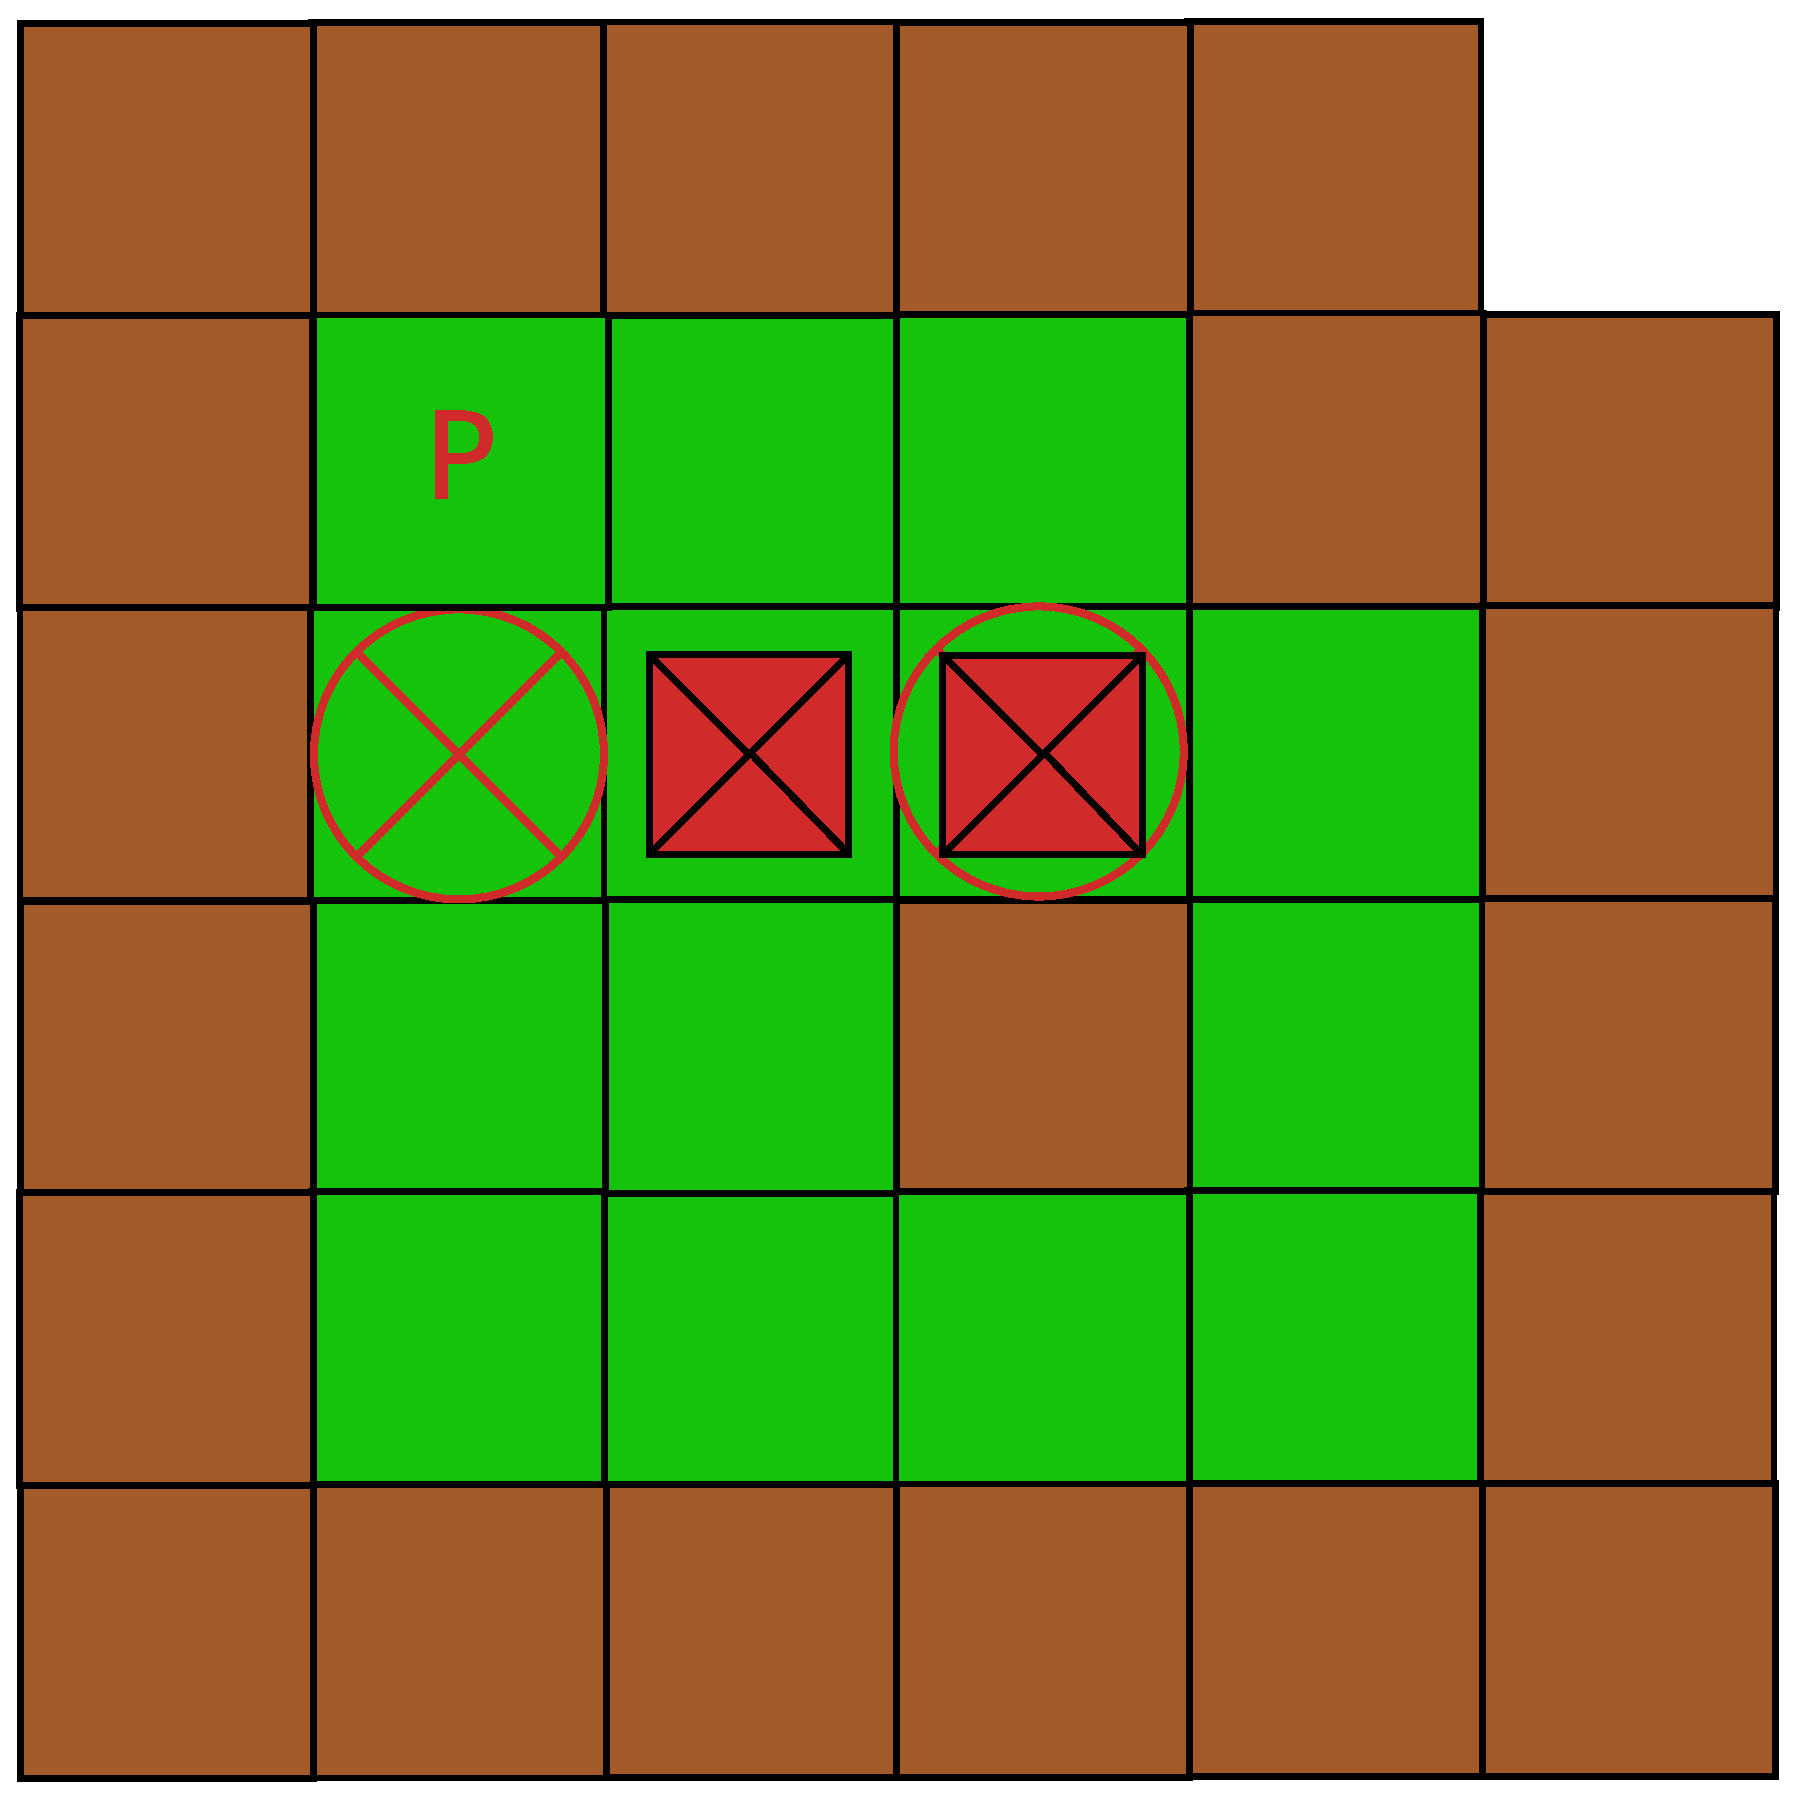
\includegraphics[scale=0.2]{Diagram1.eps}  
	\caption{
			Exemple d'une grille type de sokoban. P symbolise le joueur, les ronds rouges sont les cases d'arrivée, et les carrés représentent les caisses.
	}
	\label{label-figure1}
\end{figure}

En ASP, une grille de sokoban est encodée en spécifiant quelles cases sont des murs, et quelles cases sont des sols avec les prédicats \emph{\textcolor{blue}{mur(X,Y)}} et \emph{\textcolor{blue}{sol(X,Y)}}. On renseigne de plus un 
prédicat \emph{\textcolor{blue}{init(X,Y)}}, ce qui nous donne la position initiale du joueur, et \emph{\textcolor{blue}{caisse\_init(Numero\_caisse,X,Y)}} nous renseignant sur les positions initiales des caisses (le premier 
argument varie de 1 à $n$ lorsque l'on a $n$ de ces caisses). Enfin, le prédicat \emph{\textcolor{blue}{arrivee(X,Y)}} symbolisera une case d'arrivée en \emph{(X,Y)}.\\ \\
J'ai fait différentes versions pour ce jeu. La plus aboutie utilise une méthode incrémentale. Pour l'importer, il nous suffit d'ajouter la commande \emph{\textcolor{blue}{\#include \textless incmode\textgreater .}}. On doit alors 
définir les sous-programmes \textbf{base}, \textbf{step(k)} et \textbf{check(k)}.\\
\begin{itemize}
	\item \textbf{base :}\\
		On déclare ici des prédicats \emph{\textcolor{blue}{perso(0,X,Y)}} et \emph{\textcolor{blue}{caisse\_a\_instant(0,X,Y)}} afin de mémoriser la position du joueur à l'étape initiale (0), ainsi que celles des caisses.\\
		\textcolor{magenta}{Pour notre exemple figure \ref{label-figure1}, on aura \emph{perso(0,2,5), caisse\_a\_instant(0,3,4)}, et \\
		\emph{caisse\_a\_instant(0,4,4).}}\\
	\item \textbf{step(k) :}\\
		On a ici besoin de prédicats \emph{\textcolor{blue}{acces\_a\_instant(k, R, C)}} pour mémoriser toutes les cases accessibles depuis la position \emph{(X,Y)} de notre joueur à une étape k donnée. Pour déterminer 
		cela, on va mettre des règles pour chaque direction spécifiant que si une case est accessible à une étape $k$ et qu'une des 4 cases voisines à celle-ci est vide (un sol sans caisse) alors cette case voisine est 
		également accessible. On doit également rajouter une règle pour dire que la case sur laquelle se trouve notre personnage à l'étape choisie est accessible (cas initial pour l'induction).\\
		\textcolor{magenta}{Pour notre exemple figure \ref{label-figure1}, toutes les cases de sol ( = vertes) ne possédant pas de caisse sont accessibles. On va donc générer 12 prédicats de la sorte pour l'étape 0.}\\
		On choisit ensuite un coup pour chaque instant à l'aide d'un agrégat. Si à un instant $k$ on a deux cases de sol $c_1$ et $c_2$ sur une même ligne ou colonne et séparées d'exactement une case avec une caisse telles 
		que l'on ait accès à $c_1$ et qu'il n'y ait pas de caisse en $c_2$, alors le personnage peut se déplacer jusqu'en $c_1$, puis pousser la caisse située entre $c_1$ et $c_2$ en $c_2$. On obtient ainsi un coup jouable 
		pour l'instant $k$. L'agrégat nous sélectionne alors un seul de ces coups, qui sera sous la forme d'un prédicat \emph{\textcolor{blue}{coup\_a\_instant(k, (R, C), (R2, C2)}}.\\
		\textcolor{magenta}{Dans notre cas figure \ref{label-figure1}, seuls deux coups sont possibles : \emph{coup\_a\_instant(1,(3,3),(3,4))} et \emph{coup\_a\_instant(1,(3,5),(3,4)).}}\\
		A partir du choix du coup, on est capable de déduire quel sera la prochaine case du personnage (celle de la caisse que l'on vient de déplacer), et on peut créer les prédicats 
		\emph{\textcolor{blue}{perso(k,X,Y)}} et \emph{\textcolor{blue}{caisse\_a\_instant(k,X,Y)}} associés à l'instant $k$.\\
		\textcolor{magenta}{Par exemple si l'on a choisi le premier des deux coups jouables, on en déduira les prédicats \emph{perso(1,3,4), caisse\_a\_instant(1,3,5)}, et \emph{caisse\_a\_instant(1,4,4).}}\\
		Enfin, on est capable de savoir si on a résolu la grille ou pas à l'aide d'un prédicat \emph{\textcolor{blue}{caisse\_pas\_place(k)}} qui est vrai s'il reste une ou plusieurs caisses à placer à l'étape $k$.\\
		\textcolor{magenta}{Ici, la caisse en \emph{(3,5)} n'est pas bien placée à l'étape 1, donc on crée le prédicat \\
		\emph{caisse\_pas\_place(1)}.}\\
	\item \textbf{check(k) :}\\
		$check(k)$ est le sous-programme qui se charge d'arrêter la recherche : si à une étape $k$ ce sous-programme est satisfiable, alors le programme s'arrêtera et renverra l'ensemble solution courant. Pour vérifier si 
		l'on a trouvé une solution à notre grille, il suffit simplement d'ajouter une contrainte \emph{\textcolor{blue}{:- caisse\_pas\_place(k)}}. En effet, s'il existe une caisse non placée le $check(k)$ ne sera pas 
		satisfiable.\\
		\textcolor{magenta}{Dans notre petit exemple, le coup de caisse qu'on a choisi fait peut-être avancer la résolution, mais ne l'a pas achevé.}\\
\end{itemize}
On récupère alors la liste des coups de caisses à faire, et on peut résoudre notre grille en comblant les coups qui déplaçaient les caisses par ceux nécessaires pour atteindre la prochaine caisse à déplacer.\\
\textcolor{magenta}{Pour l'exemple figure \ref{label-figure1}, ASP nous renvoie la liste de coups suivante : s(1,(3,5),bas), s(2,(5,4),gauche), s(3,(4,4),gauche), s(4,(2,5),bas), s(5,(3,2),haut), s(6,(2,4),droite), s(7,(2,2),haut). 
\emph{s(k, case, direction)} signifie que le personnage peut aller à l'instant $k$ à la case indiquée, et pousser une caisse dans la direction indiquée.}

\section{Formalismes d'automates et leur dynamique}
Différents modèles existent pour représenter efficacement un système biologique et manipuler sa dynamique : les deux principaux sont les réseaux booléens synchrones de Stuart Kauffman, et les réseaux asynchrones de René Thomas.
Dans le cadre de mon stage je ne parlerai que des réseaux asynchrones, et plus particulièrement des réseaux d'automates asynchrone (AAN) [\cite{folschette2015sufficient}] et [\cite{pauleve2016pint}], qui forment une extension d'une précédente 
structure appelé "Process Hitting" [\cite{pauleve14}].\\

\subsection{AAN et leur traduction en ASP}
Un automate $A$, dans le contexte de mon stage, sera défini comme étant un ensemble d'états $q_0, q_1, ..., q_{|A|-1}$ avec des transitions dont les étiquettes seront un ou plusieurs états (qu'on appellera également \emph{niveaux}) 
d'automates externes. Il n'y a donc ni état final, ni état initial. On ne lui donnera pas non plus de mot à lire en entrée puisqu'on va s'intéresser à la dynamique de nos ensembles d'automates. On parlera alors de 
transition locale : $q_i\xrightarrow{l}q_j$ symbolisera le fait que l'on peut passer de l'état $q_i$ à l'état $q_j$ si toutes les conditions de $l$ sont vérifiés.\\
Un réseau d'automates asynchrone est un triplet $(\Sigma,S,T)$ avec :
\begin{itemize}
	\item $\Sigma=\left\{a,b,...\right\}$ est un ensemble fini d'automates non vides.
	\item Si $C_a$ est le nombre d'états d'un automate $a$, alors $S_a=\left\{a_0,a_1,...,a_{C_a-1}\right\}$ est l'ensemble des \textbf{états locaux} de l'automate $a$. $S=\displaystyle{\prod_{a\in\Sigma}}S_a$ est l'ensemble 
	fini des \textbf{états globaux}, et $LS=\displaystyle{\bigcup_{a\in\Sigma}}S_a$ représente l'ensemble de tous les états locaux.
	\item Pour chaque $a\in\Sigma$, $T_a\subseteq\left\{a_i\xrightarrow{l}a_j\in S_a\times\rho(LS/S_a)\times S_a|a_i\neq a_j\right\}$ est l'ensemble des \textbf{transitions locales} d'un automate $a$, avec 
	$\rho$ qui désigne la puissance ensembliste. $T=\displaystyle{\bigcup_{a\in\Sigma}}T_a$ est l'ensemble des transitions locales du modèle.\\ \\
\end{itemize}
\hypertarget{exemple}{\textbf{Exemple :}} On représente l'AAN suivant de cette manière :
\begin{itemize}
	\item $\Sigma =\left\{a,b,c\right\}$
	\item $S_a=\left\{a_0,a_1,a_2\right\}$, $S_b=\left\{b_0,b_1\right\}$ et $S_c=\left\{c_0,c_1,c_2\right\}$
	\item $T_a = \left\{a_0\xrightarrow{b_0}a_1,a_0\xrightarrow{b_1,c_1}a_1,a_1\xrightarrow{b_1}a_0,a_1\xrightarrow{b_0}a_2,a_2\xrightarrow{b_1}a_1\right\}$\\
	$T_b=\left\{b_0\xrightarrow{c_0}b_1,b_1\xrightarrow{a_2}b_0\right\}$\\
	$T_c=\left\{c_0\xrightarrow{b_1}c_1,c_0\xrightarrow{a_2}c_2,c_1\xrightarrow{b_0}c_0,c_1\xrightarrow{a_1}c_2,c_2\xrightarrow{b_1}c_0\right\}$
\end{itemize}

\begin{figure}[!h]
	\centering  
	\begin{tikzpicture}[apdotsimple/.style={apdot}]
	  \TSort{(0,2)}{a}{3}{r}
	  \TSort{(2.5,0)}{b}{2}{r}
	  \TSort{(5,2)}{c}{3}{r}

	  \path[local transitions]
	    (a_0) edge node[auto] {$b_0$} (a_1)
	    (a_1) edge node[auto] {$b_0$} (a_2)
	    (a_2) edge node[auto] {$b_1$} (a_1)
	    (a_1) edge node[auto] {$b_1$} (a_0)

	    (b_0) edge node[auto] {$c_0$} (b_1)
	    (b_1) edge node[auto] {$a_2$} (b_0)

	    (c_0) edge node[auto] {$b_1$} (c_1)
	    (c_1) edge node[auto] {$b_0$} (c_0)
	    (c_1) edge node[auto] {$a_1$} (c_2)
	    ;
	  \path[local transitions, bend left = 105]
	      (a_0) edge node[auto] {$b_1, c_1$} (a_1)
	    ;
	  \path[local transitions, bend left = 90]
	      (c_0) edge node[auto] {$a_2$} (c_2)
	    ;
	  \path[local transitions, bend left = 90]
	      (c_2) edge node[auto] {$b_1$} (c_0)
	    ;

	  \TState{a_0, b_1, c_1}
	\end{tikzpicture}
	
	\caption{Exemple de réseau d'automates asynchrone}
	\label{label-figure2}
\end{figure}



En ASP, on définira un AAN en deux temps :
\begin{itemize}
	\item On commencera par déclarer chacun de nos automates avec les niveaux (= états) qu'il contient :\\
	\emph{
		\textcolor{blue}{
		automaton\_level("a", 0..2).\\
		automaton\_level("b", 0..1).\\
		automaton\_level("c", 0..2).\\
		}
	}
	\item Enfin, les transitions seront encodés via des labels (t1, t2, ...), et on donnera chacune des conditions, ainsi que l'état d'arrivée, via un fait :\\
	\emph{
		\textcolor{blue}{
		condition(t1, "a", 0). target(t1, "a", 1). condition(t1, "b", 0).\\
		condition(t2, "a", 1). target(t2, "a", 2). condition(t2, "b", 0).\\
		condition(t3, "a", 2). target(t3, "a", 1). condition(t3, "b", 1).\\
		condition(t4, "a", 1). target(t4, "a", 0). condition(t4, "b", 1).\\
		\verb![...]!\\
		%condition(t5, "b", 0). target(t5, "b", 1). condition(t5, "c", 0).\\
		%condition(t6, "b", 1). target(t6, "b", 0). condition(t6, "a", 2).\\
		%condition(t7, "c", 0). target(t7, "c", 1). condition(t7, "b", 1).\\
		%condition(t8, "c", 1). target(t8, "c", 0). condition(t8, "b", 0).\\
		%condition(t9, "c", 1). target(t9, "c", 2). condition(t9, "a", 1).\\
		%condition(t10, "c", 0). target(t10, "c", 2). condition(t10, "a", 2).\\
		%condition(t11, "c", 2). target(t11, "c", 0). condition(t11, "b", 1).\\
		condition(t12, "a", 0). target(t12, "a", 1). condition(t12, "b", 1). condition(t12, "c", 1).\\
		}
	}
\end{itemize}
Nous avons ainsi défini l'automate de notre \hyperlink{exemple}{\textbf{exemple}} en ASP.

\subsection{Sémantiques}
\hypertarget{semantiques}{Soit $R = (\Sigma,S,T)$ un AAN (défini ci-dessus). On définit la notion de transition jouable:}
\begin{itemize}
	\item On dit qu'une transition locale est \textbf{jouable} si toutes les conditions de celle-ci sont vérifiés.\\
	On notera $P_{\zeta}$ l'ensemble des transitions locales jouables depuis un état global $\zeta$.\\
	\emph{L'état global $(a_0,b_1,c_1)$ de l'\hyperlink{exemple}{\textbf{exemple}} admet une seule transition jouable : $a_0\xrightarrow{b_1,c_1} a_1$.}
\end{itemize}
La dynamique d'un AAN se définit à l'aide de sa \textbf{sémantique}. La sémantique forme l'ensemble des propriétés définissant les \textbf{transitions globales jouables} : dans un AAN on s'intéresse à l'évolution globale du réseau.
\subsubsection{Asynchrone}
Soit $R = (\Sigma,S,T)$ un AAN, et $\zeta\in S$ un état global. L'ensemble des transitions globales jouables depuis $\zeta$ pour la sémantique \emph{asynchrone} est donnée par :
\begin{center}
	$U^{asyn}(\zeta)=\left\{\left\{a_i\xrightarrow{l} a_j\right\}|a_i\xrightarrow{l} a_j\in P_{\zeta}\right\}$
\end{center}
De manière informelle : chaque transition locale jouable est une transition globale.\\ \\
En ASP, on définit préalablement les états globaux à l'aide d'un prédicat de la forme \emph{\textcolor{blue}{global\_state(Gs)}} avec $Gs$ qui s'écrit en ASP à l'aide d'une constante unique (g1\_1\_0 symbolisera par exemple que "a" 
est au niveau 1, "b" au niveau 1 et "c" au niveau 0, cf \hyperlink{partie4.4}{Partie 4.4}). On peut ensuite déclarer que deux états globaux sont différents sur un automate à l'aide de la règle suivante :\\
\emph{
1. \textcolor{blue}{different\_on(Gs1, Gs2, Automaton) :-} \% Cet atome est vrai\\
2.\qquad \textcolor{blue}{global\_state(Gs1), global\_state(Gs2), Gs1 != Gs2,} \% si deux états globaux diffèrent\\
3.\qquad \textcolor{blue}{automaton(Automaton),} \% qu'il existe un automate\\
4.\qquad \textcolor{blue}{active\_in\_g(level(Automaton, LevelI), Gs1),} \% sur lequel $Gs1$ vaut $I$\\
5.\qquad \textcolor{blue}{active\_in\_g(level(Automaton, LevelJ), Gs2),} \% et sur lequel $Gs2$ vaut $J$\\
6.\qquad \textcolor{blue}{LevelI != LevelJ.} \% avec $I \neq J$\\ \\
}
Ensuite, on fait comprendre à ASP qu'une transition locale n'est pas jouable si l'une (au moins) de ses conditions n'est pas vérifiée de la façon suivante :\\
\emph{
1. \textcolor{blue}{unplayable(Transition, Gs) :-} \% Cet atome est vrai\\
2.\qquad \textcolor{blue}{local\_transition(Transition),} \% s'il existe une transition locale\\
3.\qquad \textcolor{blue}{global\_state(Gs),} \% un état global\\
4.\qquad \textcolor{blue}{automaton(Automaton),} \% et un automate\\
5.\qquad \textcolor{blue}{active\_in\_g(level(Automaton, LevelI), Gs),} \% sur lequel $Gs$ vaut $I$\\
6.\qquad \textcolor{blue}{condition(Transition, Automaton, LevelJ),} \% alors qu'il devrait valoir $J\neq I$\\
7.\qquad \textcolor{blue}{LevelI != LevelJ.} \% pour que la transition soit jouable\\ \\
}
On déclare ensuite que deux états globaux différent sur au moins un autre automate qu'$Automaton$ avec le terme $not\_equal\_except(Automaton, Gs1, Gs2)$ comme ceci :\\
\emph{
1. \textcolor{blue}{not\_equal\_except(Automaton, Gs1, Gs2) :-} \% Cet atome est vrai\\
2.\qquad \textcolor{blue}{automaton(Automaton), automaton(Automaton2),} \% s'il existe deux automates\\
3.\qquad \textcolor{blue}{Automaton != Automaton2,} \% qui différent\\
4.\qquad \textcolor{blue}{global\_state(Gs1), global\_state(Gs2),} \% deux états globaux\\
5.\qquad \textcolor{blue}{different\_on(Gs1, Gs2, Automaton2).} \% tels que $Gs1 \neq Gs2$ sur Automaton2\\ \\
}
On peut enfin définir ce qu'est une transition globale jouable à l'aide de nos trois précédentes règles :\\
\emph{
1. \textcolor{blue}{playable(Gs1, Gs2) :-} \% Cet atome est vrai\\
2.\qquad \textcolor{blue}{global\_state(Gs1), global\_state(Gs2),} \% s'il existe deux états globaux $Gs1$ et $Gs2$\\
3.\qquad \textcolor{blue}{automaton(Automaton), local\_transition(Transition),} \% un automate et une transition\\
4.\qquad \textcolor{blue}{target(Transition, Automaton, LevelJ),} \% qui fait changer le niveau de l'automate\\
5.\qquad \textcolor{blue}{not unplayable(Transition, Gs1),} \% et avec la transition (locale) qui est jouable\\
6.\qquad \textcolor{blue}{not not\_equal\_except(Automaton, Gs1, Gs2),} \% et $Gs1=Gs2$ excepté sur Automaton\\
7.\qquad \textcolor{blue}{active\_in\_g(level(Automaton, LevelI), Gs1),} \% tel que le niveau d'$Automaton$ dans $Gs1$\\
8.\qquad \textcolor{blue}{active\_in\_g(level(Automaton, LevelJ), Gs2),} \% et celui dans $Gs2$\\
9.\qquad \textcolor{blue}{LevelI != LevelJ.} \% sont différents\\
}
\subsubsection{Synchrone}
Soit $R = (\Sigma,S,T)$ un AAN, et $\zeta\in S$ un état global. L'ensemble des transitions globales jouables depuis $\zeta$ pour la sémantique \emph{synchrone} est donnée par :
\begin{center}
	$U^{syn}(\zeta)=\left\{u\subseteq T|u \neq \emptyset \wedge \forall a\in\Sigma,(P_{\zeta}\bigcap T_a = \emptyset \Rightarrow u\bigcap 
	T_a=\emptyset)\wedge(P_{\zeta}\bigcap T_a\neq\emptyset\Rightarrow |u\bigcap T_a |=1\right\}$
\end{center}
De manière informelle : tous les automates possédant au moins une transition locale jouable doivent changer de niveau.\\ \\
Pour coder cela en ASP, on peut se servir des atomes \emph{\textcolor{blue}{different\_on}} et \emph{\textcolor{blue}{unplayable}}.\\
On ajoute de plus une autre règle : \emph{\textcolor{blue}{has\_playable(Automaton, Gs, LevelI, LevelJ)}} spécifiant que l'on peut faire changer $Automaton$ dans $Gs$ du niveau $I$ vers le niveau $J$.\\
Enfin, il ne nous reste plus qu'a déclarer (par la négation) quelles sont les transitions globales qui ne sont pas jouables. Pour cela, on essaie pour toutes les paires d'états globaux si on peut faire la transition de l'un à 
l'autre en créant un terme \emph{\textcolor{blue}{not\_playable(Gs1,Gs2)}} si la transition ne peut pas avoir lieu. On énumère alors les différents cas de figure :
\begin{enumerate}
	\item si $Automaton$ n'admet aucune transition locale jouable dans $Gs_1$ et que $Gs_1\neq Gs_2$ sur $Automaton$
	\item si $Automaton$ admet une (ou plusieurs) transition locale jouable dans $Gs_1$ et qu'il n'existe pas de transition pour faire passer le niveau d'$Automaton$ sur $Gs_1$ à celui de $Gs_2$
	\item si aucune transition locale n'est jouable depuis $Gs_1$
\end{enumerate}
alors la transition $Gs_1\rightarrow Gs_2$ n'est pas jouable.\\
Enfin, il nous suffit de tester pour toutes les paires d'états globaux distincts si on a \emph{\textcolor{blue}{not\_playable(Gs1,Gs2)}} ou pas. Dans le cas contraire, alors on crée l'atome 
\emph{\textcolor{blue}{playable(Gs1,Gs2)}}.

\subsubsection{Généralisée}
Soit $R = (\Sigma,S,T)$ un AAN, et $\zeta\in S$ un état global. L'ensemble des transitions globales jouables depuis $\zeta$ pour la sémantique \emph{généralisée} est donnée par :
\begin{center}
	$U^{gen}(\zeta)=\left\{u\subseteq T|u \neq \emptyset \wedge \forall a\in\Sigma,(P_{\zeta}\bigcap T_a = \emptyset \Rightarrow u\bigcap 
	T_a=\emptyset)\wedge(P_{\zeta}\bigcap T_a\neq\emptyset\Rightarrow |u\bigcap T_a |\leq 1\right\}$
\end{center}
De manière informelle : tous les automates possédant au moins une transition locale jouable \underline{peuvent} changer de niveau, et au moins l'un d'entre eux doit changer de niveau.\\ \\
Pour coder cela en ASP, on prend exactement le code de la sémantique synchrone, en remplaçant le second cas de figure par ceci :\\ \\
\textcolor{white}{4cha}2. si $Gs_1$ différe de $Gs_2$ sur $Automaton$ et qu'il n'existe pas de transition pour faire passer 
\textcolor{white}{6chara}le niveau d'$Automaton$ sur $Gs_1$ à celui de $Gs_2$\\ \\
Cela permet bien de ne pas prendre une transition par automate qui est jouable puisqu'on va tester des paires d'états globaux qui ont peut-être 3 automates jouables, et si l'on ne fait qu'une seule transition locale cela ne sera pas 
filtré par notre atome \emph{\textcolor{blue}{not\_playable(Gs1,Gs2)}}.

\subsection{Dynamique}
Soit $U$ une sémantique. On introduit les dernières notions nécessaires pour la définition d'un attracteur :
\begin{itemize}
	\item On appelle \textbf{état stable} un état global ne possédant aucune transition globale jouable pour $U$.
	\emph{Dans l'\textbf{exemple}, aucun état global n'est stable pour la sémantique asynchrone (et donc cela est également vrai pour la sémantique synchrone et généralisée).}
	\item Pour $Gs_1,Gs_2\in S$, on notera $Gs_1\rightarrow _UGs_2$ pour symboliser le fait qu'il existe $u\in U(Gs_1)$ tel que si l'on joue toutes les transitions locales de $u$, alors $Gs_1$ devient $Gs_2$.
	\item Un \textbf{chemin} est une famille finie $(A_k)_{1\leq k\leq n}$ et ordonnée d'états globaux tels que pour tout $1\leq k\leq n-1$, $A_k\rightarrow _U A_{k+1}$.
	\item Un \textbf{cycle} est un chemin $(A_k)_{1\leq k\leq n}$ tel que $A_1=A_n$.
	\item Un \textbf{domaine de piège} est un ensemble non vide d'états globaux $S_E\in S$ tel que toute transition globale jouable depuis $S_E$ arrive dans un état global de $S_E$. Plus formellement : 
	$\forall\zeta _1\in S_E \wedge\forall\zeta _2\in S, \zeta _1 \rightarrow _U\zeta _2 \Rightarrow\zeta _2\in S_E$
\end{itemize}
Enfin, on peut définir ce qu'est un attracteur.\\
Un ensemble $A\subseteq S$ d'états globaux, avec $|A|\geq2$ est appellé \textbf{attracteur} si et seulement si c'est un domaine de piège minimal en terme d'inclusion ensembliste.\\
\cite{chapitre} a démontré le résultat mathématique suivant dont on va se servir pour trouver les attracteurs au sein d'un AAN :\\ \\
\textbf{Lemme :} Les attracteurs d'un AAN sont exactement les domaines de piège cycliques.

\section{Cœur de la contribution personnelle}
\hypertarget{debutpartie4}{
La version de laquelle j'ai commencé à travailler est assez proche du travail que j'ai effectué. Cette version était fonctionnelle et efficace pour la sémantique asynchrone, mais ne fonctionnait pour la sémantique synchrone que 
lorsque les attracteurs étaient exactement des cycles simples (chaque état global du graphe produit doit avoir un degré sortant égal à $1$), et ne fonctionnait pas pour les autres AAN comme celui-ci :\\ \\ \\
}

\begin{figure}[!h]
	\centering  
	\begin{tikzpicture}[apdotsimple/.style={apdot}]

	  \TSort{(0,2)}{a}{3}{r}
	  \TSort{(3,2)}{b}{3}{r}

	  \path[local transitions]
	    (a_0) edge node[auto] {$b_0$} (a_1)
	    (a_1) edge node[auto] {$b_1$} (a_2)
	    (a_2) edge node[auto] {$b_1$} (a_1)

	    (b_0) edge node[auto] {$a_0$} (b_1)
	    (b_1) edge node[auto] {$a_1$} (b_2)
	    (b_2) edge node[auto] {$a_1$} (b_1)
	    ;
	    
	    \path[local transitions, bend left = 90]
	      (a_0) edge node[auto] {$b_0$} (a_2)
	    ;
	    \path[local transitions, bend left = 90]
	      (a_2) edge node[auto] {$b_2$} (a_0)
	    ;
	    \path[local transitions, bend left = 90]
	      (b_0) edge node[auto] {$a_0$} (b_2)
	    ;
	    \path[local transitions, bend left = 90]
	      (b_2) edge node[auto] {$a_2$} (b_0)
	    ;
	\end{tikzpicture} 
	\caption{Exemple d'AAN sur lequel le code pré-existant ne trouvait pas l'attracteur}
	\label{label-figure3}
\end{figure}

\begin{figure}[!h]
	\centering  
	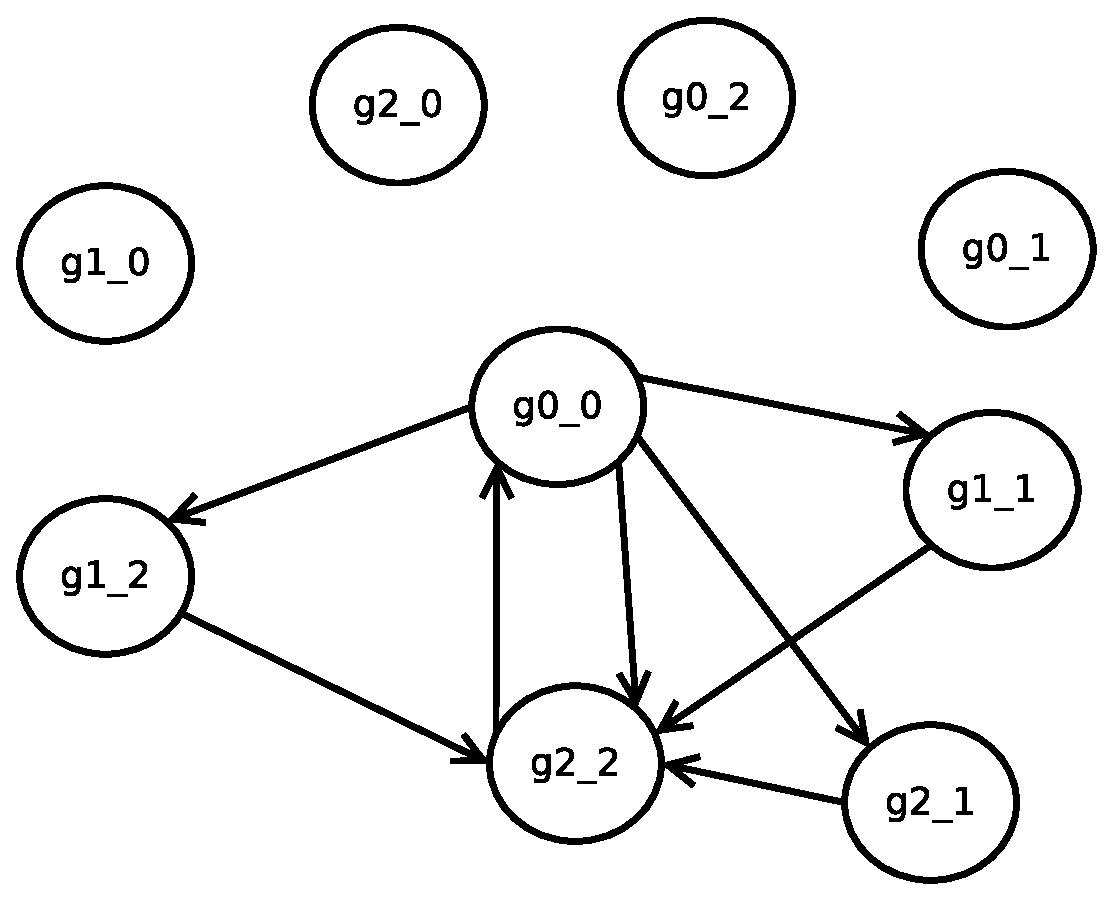
\includegraphics[scale=0.3]{Diagram2.eps}  
	\caption{Graphe produit de l'AAN ci-dessus}
	\label{label-figure4}
\end{figure}

En effet, l'ensemble $\left\{(0,0),(1,1),(1,2),(2,1),(2,2)\right\}$ est un attracteur de cet AAN pour la sémantique synchrone. De plus, il existe deux (même quatre ici) transitions globales jouables depuis l'état global $(0,0)$ : 
on peut aller en $(1,1)$ ou encore en $(2,2)$.\\ \\
Après avoir identifié le problème au sein du code, j'ai trouvé deux alternatives pour corriger cela : la première consiste à reprendre tout le code, enlever le problème ciblé et corriger cela avec un script Python, et la seconde 
consiste à considérer les états globaux et à définir les transitions globales jouables dans des fichiers dédiés aux sémantiques. Je vais donc détailler deux manières de trouver les attracteurs d'un AAN en ASP.

\subsection{Code pré-existant}
\hypertarget{preexistante}{On explique tout d'abord comment générer des chemins d'une longueur définie dans un AAN.}\\ \\
\emph{
	\% On mémorise quelques informations : noms des automates et des transitions locales\\
	1. \textcolor{blue}{automaton(Automaton) :- automaton\_level(Automaton, \_).}\\
	2. \textcolor{blue}{local\_transition(Transition, Automaton) :- target(Transition, Automaton, \_).}\\
	3. \textcolor{blue}{local\_transition(Transition) :- target(Transition, \_, \_).}\\ \\
	\% On définit ensuite les étapes de notre chemin\\
	4. \textcolor{blue}{step(0..n).} \% Ici n est une constante qu'on définit lors de la compilation (souvent 10)\\
	5. \textcolor{blue}{1 \{main\_cycle\_length(N) : step(N), N \textgreater 0 \} 1.}\% La longueur du cycle principal\\
	6. \textcolor{blue}{cycle\_step(0..N) :- main\_cycle\_length(N).}\% On nomme les étapes du cycle principal\\
	7. \textcolor{blue}{after\_cycle\_step(N+1..n) :- main\_cycle\_length(N).}\% différemment de celles d'après\\ \\
	\% On choisit ensuite un état initial à l'aide d'un agrégat\\
	8. \textcolor{blue}{1 \{ active(level(Automaton, Level), 0) : automaton\_level(Automaton, Level) \} 1 :-}\\
	9.\qquad\qquad\textcolor{blue}{automaton(Automaton).}\\ \\
	\% On calcule les transitions locales non jouables pour chaque étape\\
	10. \textcolor{blue}{unplayable(Transition, Step) :-}\\
	11.\qquad\qquad\textcolor{blue}{active(level(Automaton, LevelI), Step),}\\
	12.\qquad\qquad\textcolor{blue}{condition(Transition, Automaton, LevelJ),}\\
	13.\qquad\qquad\textcolor{blue}{LevelI != LevelJ, step(Step).}\\ \\
	\% On trouve les automates qui ont au moins une transition jouable (sémantique synchrone)\\
	14. \textcolor{blue}{has\_playable(Automaton, Step) :-}\\
	15.\qquad\qquad\textcolor{blue}{not unplayable(Transition, Step),}\\
	16.\qquad\qquad\textcolor{blue}{local\_transition(Transition, Automaton),}\\
	17.\qquad\qquad\textcolor{blue}{step(Step).}\\ \\
	\% On sélectionne une transition à jouer pour chaque automate si possible\\
	18. \textcolor{blue}{1 \{played(Transition, Step) :}\\
	19.\qquad\qquad\textcolor{blue}{not unplayable(Transition, Step),}\\
	20.\qquad\qquad\textcolor{blue}{local\_transition(Transition, Automaton)}\\
	21. \textcolor{blue}{\} 1 :- has\_playable(Automaton, Step).}\\ \\
	\% Contrainte : on doit jouer au moins une transition locale à chaque étape\\
	22. \textcolor{blue}{:- 0 \{ played(\_, Step) \} 0, step(Step).}\\ \\
	\% Maintenant que l'on a choisi notre coup, on en déduit le changement à faire.\\
	23. \textcolor{blue}{change(Transition, Automaton, LevelI, LevelJ, Step) :-}\\
	24.\qquad\qquad\textcolor{blue}{played(Transition, Step),}\\
	25.\qquad\qquad\textcolor{blue}{target(Transition, Automaton, LevelJ),}\\
	26.\qquad\qquad\textcolor{blue}{condition(Transition, Automaton, LevelI).}\\ \\
	\% On change le niveau actif s'il y a un changement dans Automaton\\
	27. \textcolor{blue}{active(level(Automaton, LevelK), Step + 1) :-}\\
	28.\qquad\qquad\textcolor{blue}{change(\_, Automaton, \_, LevelK, Step),}\\
	29.\qquad\qquad\textcolor{blue}{Step \textless n.}\\ \\
	\% On garde le niveau actif s'il n'y a pas de changement dans Automaton\\
	30. \textcolor{blue}{active(level(Automaton, LevelK), Step + 1) :-}\\
	31.\qquad\qquad\textcolor{blue}{not change(\_, Automaton, \_, \_, Step),}\\
	32.\qquad\qquad\textcolor{blue}{active(level(Automaton, LevelK), Step),}\\
	33.\qquad\qquad\textcolor{blue}{step(Step), Step \textless n.}\\ \\
}
Je viens ici d'expliquer comment faire pour générer tous les chemins de longueur $n$ avec la sémantique synchrone. Cependant, pour qu'un de ses chemins nous intéresse, il faut qu'il respecte les 3 contraintes suivantes :\\
\begin{itemize}
	\item avoir un cycle de longueur N (lorsque \emph{\textcolor{blue}{main\_cycle\_length(N)}} est vrai)
	\item tout les états globaux du chemin visités après l'étape N (lorsque \emph{\textcolor{blue}{main\_cycle\_length(N)}} est vrai) doivent être des éléments du cycle
	\item toutes les transitions globales jouables depuis chacun des éléments du cycle doivent arriver dans un autre élément de ce cycle ( = domaine piège)\\
\end{itemize}
Les deux premières conditions se vérifient assez aisèment.\\ \\
Pour la première, on crée un prédicat \textcolor{blue}{\emph{different\_states\_on(Step1, Step2, Automaton)}} nous permettant de déduire si deux états globaux atteints à $Step_1$ et $Step_2$ sont différents ou pas. On en déduit 
alors un prédicat \textcolor{blue}{\emph{same\_state(Step1, Step2)}}, et il ne nous reste qu'à ajouter la contrainte \textcolor{blue}{\emph{:- not same\_state(0, N), main\_cycle\_length(N).}}\\ \\
Quant à la seconde, il nous suffit de créer un prédicat \textcolor{blue}{\emph{valid\_state\_after\_main\_cycle(Step2)}} vrai lorsqu'il existe une étape $Step_1$ dans le cycle principal et une étape $Step_2$ en dehors du cycle 
principal telles que l'on ait l'atome \textcolor{blue}{\emph{same\_state(Step1, Step2)}} qui soit vrai. Ce prédicat devant être toujours vrai pour chaque $Step_2$, on rajoute finalement la contrainte suivante :\\
\textcolor{blue}{\emph{:- not valid\_state\_after\_main\_cycle(Step1), after\_cycle\_step(Step1).}}\\ \\
La troisième contrainte contenait la raison du bug du code (cf début \hyperlink{debutpartie4}{partie 4}). Comme la modélisation actuelle des choses ne mémorise pas quels sont les coups jouables pour la sémantique choisie 
(cela permettait d'avoir un code qui fonctionne pour toutes les sémantiques en scindant le fichier ASP en deux : recherche des attracteurs, et sémantique, ce qui permettait d'avoir un seul solveur d'attracteur, universel 
pour toutes les sémantiques), cela n'était pas possible. Deux options étaient alors envisageables pour résoudre ce problème : faire un script ASP dans laquelle je rajoute la dernière contrainte en introduisant une notion d'état 
global ; ou bien utiliser Python pour résoudre ce problème lors du solving de clingo.

\subsection{Résolution de la troisième contrainte en Python}
Je ne vais pas rentrer en détail dans la manière dont on peut réussir à récupérer des atomes lors du grounding et du solving d'ASP en Python : on admettra que cela est faisable. Nous avons donc en Python une 
\textcolor{blue}{\emph{boucle for}} qui va, à chaque instance, avoir un ensemble d'atomes tous vrais tel que l'interprétation qu'ils forment satisfasse toutes les règles de notre programme ASP.\\ \\
Lors de la première itération de cette boucle, il est nécessaire de mémoriser toutes les transitions, les conditions, ainsi que les cibles de ces transitions. On introduit donc quelques ensembles pour stocker cela en mémoire.\\ \\
\emph{
	1. \textcolor{blue}{condition\_transitions = \{\}} \# de la forme [transition][automata] = level\\
	2. \textcolor{blue}{target\_transitions\_automaton\_name = \{\}} \# de la forme [transition] = automaton\_name\\
	3. \textcolor{blue}{target\_transitions\_automaton\_level = \{\}}  \# de la forme [transition] = level\\
	4. \textcolor{blue}{transitions\_already\_done = False}\\ \\
}
Ensuite, dès le début de la \emph{\textcolor{blue}{boucle for}} magique, on récupère toutes les informations nécessaires pour remplir ces ensembles, et on modifie la variable booléenne \emph{\textcolor{blue}
{transitions\_already\_done}} à True afin de ne plus faire cela lors des autres itérations de la boucle.\\
On en profite également pour créer un ensemble \emph{\textcolor{blue}{cur\_set}}  de la forme \emph{\textcolor{blue}{[step\_number][automata\_name] = active\_level}} qui viendra mémoriser les états globaux de chaque étape de 
l'ensemble solution courant.\\ \\
Ensuite, on crée un ensemble \emph{\textcolor{blue}{playable}} qu'on va venir remplir avec les transitions locales jouables depuis chacun des états globaux de l'attracteur courant et chaque automate de ce dernier. Il est de la forme 
\emph{\textcolor{blue}{playable[global\_state][automata\_name][transition] = level}} où 'level' est le niveau de l'automate après la transition. Pour remplir ce dernier, il faut qu'on teste pour chaque transition locale si elle est 
jouable pour l'état global courant ou pas en regardant pour chaque condition de la transitions si elle est vérifiée ou pas. Si elle est bien jouable, on l'ajoute au dictionnaire.\\ \\
On se sert de l'ensemble \emph{\textcolor{blue}{playable}} pour créer une liste de listes de listes d'entiers \emph{\textcolor{blue}{list\_of\_list}}.Pour faire simple, chacune de ses sous-listes représente un état global de 
l'attracteur courant. Chacune des sous-listes de ces états globaux représente un automate, et chacune des sous-listes de cet automate correspond à l'ensemble des niveaux dans lesquels il peut se retrouver après une transition locale 
jouable depuis l'état global. Si aucune transition locale n'est jouable, la sous-liste de l'automate en question sera vide. Pour remplir cette liste, on procède de la façon suivante :\\
\begin{itemize}
	\item Pour chaque état global de l'attracteur courant on crée une liste \emph{\textcolor{blue}{list\_for\_current\_state}} (des automates)
	\item Pour chaque automate de cet état global on crée une liste \emph{\textcolor{blue}{list\_for\_automaton}}(des niveaux atteignables)
	\item Si aucune transition locale n'est jouable pour l'automate, on le laisse à son niveau
	\item Sinon pour chaque transition locale jouable on détermine le niveau après transition de l'automate et on l'ajoute à la liste des niveaux atteignables de l'automate
	\item on ajoute la liste des niveaux atteignables de l'automate à l'état global, puis la liste de l'état global à \emph{\textcolor{blue}{list\_of\_list}}\\
\end{itemize}
L'utilisation d'une liste de listes est très pratique puisqu'il nous suffit alors d'effectuer un produit cartésien de listes pour en déduire les listes de tout les états globaux atteignables depuis notre attracteur courant. C'est 
exactement ce qu'on calcule dans \emph{\textcolor{blue}{list\_of\_product}} : la liste des produits cartésiens de chaque coup possible pour un état global.\\ \\
Enfin, il nous suffit de vérifier que chaque élément de list\_of\_product est bien un élément du cycle principal. De cette façon, notre attracteur vérifiera bien la troisième condition, et sera valide.
Si un au moins des éléments de \emph{\textcolor{blue}{list\_of\_product}} n'est pas dans l'attracteur, alors il ne s'agit en réalité pas d'un attracteur : on peut s'en échapper.\\ \\
C'est ici que l'on termine la \emph{\textcolor{blue}{boucle for}} magique.\\ \\
Les résultats de cette version sont plus qu'appréciables. En effet, j'ai utilisé la même batterie de tests que Maxime Folschette pour la version de laquelle je suis parti, et les durées de résolution se sont avérées toutes aussi 
bonnes que celles de la sémantique asynchrone.

\subsection{Légère modification pour sémantique généralisée}
En reprenant le code présenté ci-dessus, j'ai également fait une version pour la sémantique généralisée (la version de laquelle je suis parti fonctionnant très bien pour la sémantique asynchrone, je n'ai rien à dire 
dessus). En effet, la différence avec la sémantique synchrone est que l'on peut faire changer nos automates ou pas, mais qu'au moins un de tous les automates doit changer de niveau lorsque l'on recherche quelles sont les 
transitions globales jouables.
Concrètement, il faut modifier la sémantique dans le code pré-existant en ASP:\\ \\
\emph{
	\textcolor{blue}{\verb![...]!}\\
	\% On sélectionne \underline{0 ou 1} transition à jouer pour chaque automate\\
	18. \textcolor{blue}{\textcolor{red}{0} \{played(Transition, Step) :}\\
	19.\qquad\qquad\textcolor{blue}{not unplayable(Transition, Step),}\\
	20.\qquad\qquad\textcolor{blue}{local\_transition(Transition, Automaton)}\\
	21. \textcolor{blue}{\} 1 :- has\_playable(Automaton, Step).}\\
	\textcolor{blue}{\verb![...]!}\\ \\
}
On doit ensuite modifier dans le code python le fait que \emph{\textcolor{blue}{list\_for\_automaton}} soit initialement vide : pour chaque automate, on peut soit rester dans cet automate, soit faire une des transitions trouvés. 
On va donc initialiser cette liste de cette façon :\\
\emph{\textcolor{blue}{list\_for\_automaton = [global\_state[sorted\_automata\_names.index(automaton\_name)]]}} (où \\
\emph{\textcolor{blue}{sorted\_automata\_names}} est une liste des noms d'automates triée par ordre lexicographique). Ensuite, on rajoute à \emph{\textcolor{blue}{list\_for\_automaton}} tous les autres niveaux atteignables pour 
l'état global courant (tout comme la sémantique synchrone).

\subsection{\'Etude des états globaux}
\hypertarget{partie4.4}{
L'autre solution que je voyais pour résoudre le problème qu'ont rencontré mon maître de stage et ses collègues était de déclarer des prédicats \emph{\textcolor{blue}{global\_state(Gs)}} représentant les états globaux du réseau. 
Cela permet de déclarer dans des fichiers pour les sémantiques quelles sont les transitions locales jouables en utilisant un prédicat \emph{\textcolor{blue}{playable(Gs1, Gs2)}} signifiant que l'on peut aller depuis 
$Gs_1$ en $Gs_2$.}\\ \\
Le principal défaut de cette manière de procéder est que cela crée de nombreux atomes et demande à ASP de les garder en mémoire pendant toute sa résolution. De plus, déterminer si pour toute paire d'états globaux il existe une 
transition se fait en $O(k^2)$, avec $k=\displaystyle{\prod_{a\in\Sigma}C_a}$, alors que si l'on calcule les transitions jouables à chaque étape, on ne surcharge pas la mémoire du solveur. C'est à priori ce qui rend mon programme 
obsolète en terme de complexité.\\ \\
Les explications d'ASP que j'ai faites pour la \hyperlink{semantiques}{partie 3.2} sur les différentes sémantiques sont en réalité mes propres fichiers pour les trois sémantiques.\\ \\
Dans cette section, je compte expliquer comment fonctionne mon fichier ASP principal, ainsi que comment je m'y suis pris pour déclarer des états globaux sans modifier la manière d'écrire un automate (en ASP on ne peut pas créer 
de tuples ayant une arité variable en fonction d'un prédicat).\\ \\
J'ai d'abord défini deux fonctions en Python permettant de créer une constante pour un état global représenté par une liste-ASP (un objet que j'introduis par la suite) : ce sera la fonction \emph{\textcolor{blue}{work(g)}}, et de 
déterminer les niveaux des automates actifs de ces constantes : ce sera la fonction \emph{\textcolor{blue}{determine\_active\_level(a,g)}} . Je ne détaillerais pas le code de ces fonctions.\\
\begin{itemize}
	\item\emph{\textcolor{blue}{work(g)}} prend un état global encodé sous forme de liste-ASP et renvoie une constante unique en ASP représentant l'état global en entrée.\\
	\item\emph{\textcolor{blue}{determine\_active\_level(a,g)}} prend un automate a sous la forme d'une chaîne de caractères, et un état global g sous la forme de sa constante en ASP, et renvoie un prédicat "level(a, 	
	niveau\_de\_a)" en ASP.
\end{itemize}
La structure du code ASP reprend fortement celle de la \hyperlink{preexistante}{version pré-existante}, c'est pourquoi je ne vais pas la mettre intégralement.\\ \\
Après avoir introduit quelques informations (noms d'autoamtes, transitions locales, étapes du chemin) comme c'est fait dans les 7 premières lignes de la version pré-existante, on introduit 2 prédicats supplémentaires utiles pour 
définir un ordre parmi les automates. On utilise alors une fonction de clingo : \#count \{E\} permettant de compter le nombre d'éléments dans l'ensemble E.\\ \\
\emph{
	8. \textcolor{blue}{nb\_automaton(N) :- N = \#count \{ A : automaton(A) \}.}\\
	9. \textcolor{blue}{nb\_level(A, N) :- automaton(A), N = \#count \{ L : automaton\_level(A, L) \}.}\\
	10. \textcolor{blue}{enum(1..N) :- nb\_automaton(N).}\\ \\
}
\`A l'aide des prédicats \emph{\textcolor{blue}{enum(k)}} que l'on vient juste de créer, on peut désormais définir un ordre pour les automates :\\ \\
\emph{
	11. \textcolor{blue}{1 \{ moment(A, N) : enum(N) \} 1 :- automaton(A).}\\
	12. \textcolor{blue}{1 \{ moment(A, N) : automaton(A) \} 1 :- enum(N).}\\
	13. \textcolor{blue}{:- }\\
	14.\qquad\textcolor{blue}{moment(A, N), moment(A2, N2),}\\
	15.\qquad\textcolor{blue}{automaton(A), automaton(A2),}\\
	16.\qquad\textcolor{blue}{enum(N), enum(N2),}\\
	17.\qquad\textcolor{blue}{N \textless N2, A \textless A2.}\\ \\
}
Une fois cet ordre défini, on est capable de créer une liste-ASP pour encode chacun des états globaux. Le $(N-k)^{ieme}$ élément de cette liste sera un prédicat nb(automaton, level) avec automaton étant $k^{ieme}$ au niveau de 
l'ordre défini précédemment (on empile dans la liste d'abord les premiers éléments, c'est pour ça qu'on a trié par ordre anti-lexicographique).\\ \\
\emph{
	18. \textcolor{blue}{build\_list(0, empty).}\\
	19. \textcolor{blue}{build\_list(N+1, (nb(A, 0..K-1), L)) :-}\\ 
	20.\qquad\textcolor{blue}{build\_list(N, L),}\\
	21.\qquad\textcolor{blue}{enum(N+1),}\\
	22.\qquad\textcolor{blue}{moment(A, N+1),}\\
	23.\qquad\textcolor{blue}{nb\_level(A, K).}\\ \\
}
On utilise ensuite nos fonctions Python pour travailler avec des constantes plus agréables à lire que des grosses listes ASP.\\ \\
\emph{
	24. \textcolor{blue}{gs(L) :- build\_list(N, L), nb\_automaton(N).}\\
	25. \textcolor{blue}{global\_state(@work(gs(L)), L) :- gs(L). }\\ 
	26. \textcolor{blue}{global\_state(Gs) :- global\_state(Gs, \_).}\\
	27. \textcolor{blue}{active\_in\_g(@determine\_active\_level(Automaton, L), Gs) :-}\\
	28.\qquad\textcolor{blue}{automaton(Automaton),}\\
	29.\qquad\textcolor{blue}{global\_state(Gs,L).}\\ \\
}
Avec tout ces éléments, il est alors très facile de poursuivre l'algorithme et de déclarer les 3 contraintes de l'attracteur comme on l'avait fait dans la version pré-existante : on choisit un état global à l'étape initiale 
(step 0), pour chaque étape on choisit un coup jouable en connaissant l'état dans lequel on se trouve à cette étape. Puis on détermine quel est l'état global de l'étape suivante, et on teste ensuite les trois contraintes avec les 
états globaux. La troisième contrainte est alors très simple à encoder maintenant que l'on a mémorisé les coups jouables dans la sémantique :\\ \\
\emph{
	30. \textcolor{blue}{also\_playable(Gs1, Gs2, Step) :-}\\
	31.\qquad\textcolor{blue}{playable(Gs1, Gs2),}\\
	32.\qquad\textcolor{blue}{not played(Gs1, Gs2, Step),}\\
	33.\qquad\textcolor{blue}{active\_g(Gs1, Step),}\\
	34.\qquad\textcolor{blue}{step(Step).}\\ \\
	35. \textcolor{blue}{evolves\_in\_main\_cycle(Gs1, Gs2, Step1, Step2) :-}\\
	36.\qquad\textcolor{blue}{playable(Gs1, Gs2),}\\
	37.\qquad\textcolor{blue}{active\_g(Gs1, Step1),}\\
	38.\qquad\textcolor{blue}{active\_g(Gs2, Step2).}\\ \\
	39. \textcolor{blue}{:- also\_playable(Gs1, Gs2, Step), not evolves\_in\_main\_cycle(Gs1, Gs2, Step, \_).}\\ \\
}
Les résultats de cette version sont décevants. Avec les mêmes tests que précédemment, je n'ai réussi à obtenir que 2 (sur 7) solutions en moins de 100s, ce qui n'est vraiment pas bon. Maxime Folschette et moi-même pensons que cela 
est dû à la trop grosse quantité de mémoire d'ASP gardé pour de trop nombreux prédicats.

\newpage
\section{Conclusion et pistes pour la suite}
Durant mon stage j'ai élaboré deux versions pour résoudre le problème rencontré avec l'ajout de la troisième contrainte. J'ai présenté dans ce rapport la solution qui fait appel à un script Python, ainsi que la version modifiée 
pour traiter la sémantique généralisée. J'ai très brièvement parlé de la solution nécessitant la création d'états globaux en ASP.\\ \\
Mes performances sur la batterie de test qu'a utilisé Maxime Folschette pour la version de laquelle je suis parti se sont avérées toutes aussi bonnes que celles de la sémantique asynchrone. Les résultats de ces tests sont 
disponibles sur le github de mon stage, juste \href{https://github.com/Leopoulpinator/Attractors-in-AAN/tree/main/versions/final_versions}{ici}. Les performances de ma seconde version y sont également. On voit notamment à quel point 
elle n'est pas efficace en temps.\\ \\
Concernant cette seconde version, je pense que l'on peut grandement améliorer son efficacité en combinant mon code avec de l'incrémental. L'idée serait de ne considérer qu'un certains nombres d'états globaux : au début on les 
considère tous, puis, lorsque l'on trouve un attracteur, on regroundre le programme en enlevant tout les états globaux de l'attracteur (en les mettant tous à faux).\\ \\
Une autre idée que j'avais en tête était, lorsque l'on trouvait un cycle qui n'était pas un attracteur, de remplacer tout les états de ce cycle par un seul représentant, dont les transitions globales entrantes et sortantes 
seront celles de chacun des états globaux du cycle. On travaillerait ensuite avec des représentants et des états globaux comme s'il s'agissait du même objet (si on a un représentant dans un autre cycle, on l'agrandira en rajoutant 
les autres éléments du cycle). Je pense que combiner cette idée avec de l'incrémental pourrait également être intéressant : à chaque cycle trouvé on effectue de nouveau un grounding en mettant à jour nos représentants.\\ \\
Je ne suis pas sûr de ces pistes, mais c'est ce sur quoi j'essaierais personnellement de me pencher pour poursuivre le travail.\\ \\ \\
Enfin, je souhaite remercier l'ENS de Lyon qui m'a proposé ce stage, Maxime Folschette pour son encadrement, les personnes au sein de l'équipe BioComputing, mes quelques collègues stagiaires de bureau (même si le stage a été en 
semi-distanciel) ainsi que mes quelques relecteurs anonymes.\\ \\
Mon code est disponible \href{https://github.com/Leopoulpinator/Attractors-in-AAN}{ici}.

\newpage
\bibliography{biblio}

\end{document}





























